\documentclass[bigger]{beamer}
\usepackage[utf8]{inputenc}
\usepackage[T1]{fontenc}
\usepackage{fontspec}
\usepackage{hyperref}
\usepackage{url}
\usepackage{booktabs}
\usepackage[utf8]{inputenc}
\defaultfontfeatures{Mapping=tex-text}

\usepackage{tikz}
\usetikzlibrary{positioning}
%\usepackage[hungarian]{babel}

\title{Introduction to Machine Learning}
\date[]{\today}
\author[Ádám Kovács]{Ádám Kovács \texttt{kovacs.adam@aut.bme.hu}}

\usetheme{aut}

\begin{document}

\begin{frame}
\titlepage
\end{frame}

\begin{frame}
    \begin{center}
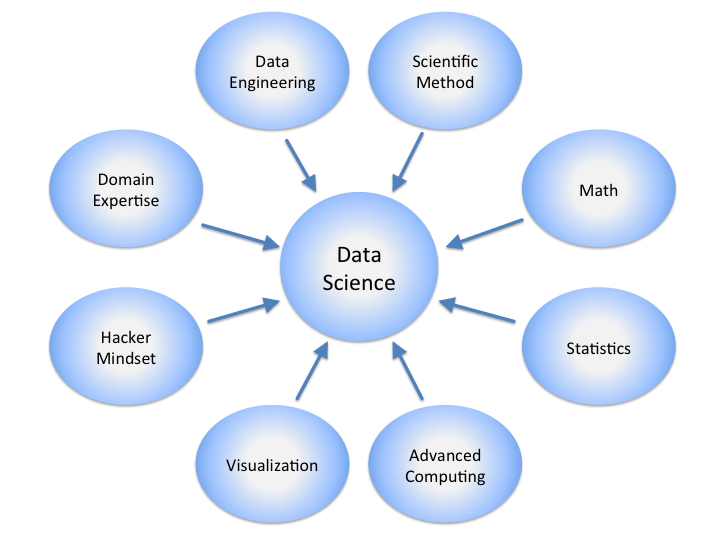
\includegraphics[width=.8\textwidth]{fig/data_science}
    \end{center}
    \footnotesize{source: wikipedia.org}
\end{frame}

\begin{frame}{Data mining}
    \begin{quote}
        The nontrivial extraction of implicit, previously
    unknown, and potentially useful information
    from data.
    \end{quote}
    \begin{itemize}
        \item non-trivial
        \item relationship between data points
        \item (large) dataset
        \item make predictions on unknown examples
    \end{itemize}
\end{frame}

\begin{frame}{Examples and counterexamples}
    Convenience store statistics
    \begin{itemize}
        \item Number of customers
            \begin{itemize}
                \item trivial information
            \end{itemize}
        \item Last month's income
            \begin{itemize}
                \item trivial information
            \end{itemize}
        \item Items most frequently bought together
            \begin{itemize}
                \item \emph{finding frequent itemsets}
            \end{itemize}
        \item How many cashiers need to be open at Friday 16 pm?
            \begin{itemize}
                \item customer queuing model
                \item \emph{time series modeling}
            \end{itemize}
    \end{itemize}
\end{frame}

\begin{frame}{Multidisciplinary field}
    \begin{description}
        \item[mathematics] linear algebra, matrix algebra, optimization, statistics, analysis
        \item[software engineering] data collection, data cleaning, employing machine learning algorightms
        \item[other] bioinformatics, computational linguistics, computational social sciences
    \end{description}
\end{frame}

\begin{frame}{Data representation 1.}
    \begin{itemize}
        \item Vector space models
            \begin{itemize}
                \item one vector corresponds to one observation or sample
                \item the number of features of the observation space is the dimension of the vectors
                \item e.g.~spam detection - one vector represents one email
                \item the dimension of the vector is optional
            \end{itemize}
    \end{itemize}
\end{frame}

\begin{frame}{Data representation 2.}
    \begin{itemize}
        \item Time series
            \begin{itemize}
                \item there exists a natural ordering of the samples
                \item doesn't have to be 'time'
                \item e.g.~daily precipitation in Budapest
                \item words in a document
            \end{itemize}
        \item Graph
            \begin{itemize}
                \item data points have explicit relationship with each other such as casual relations
                \item e.g.~modeling medical problems, diseases (What causes cancer?)
                \item geographic relationship: traffic in Budapest
            \end{itemize}
    \end{itemize}
    Choosing the right representation is crucial.
\end{frame}

\begin{frame}{Vector representation}
    \begin{description}
        \item[sample] one data point - \textcolor{darkred}{vector}
        \item[feature] a property or attribute of a sample - \textcolor{darkred}{one element of a vector}
		 \begin{itemize}
			\item length of the mail
			\item sender
			\item Does it contain the word \emph{Rolex}?
			\item Does it contain the expression \emph{Trust fund}?
		\end{itemize}
        \item[dataset] collections of all samples - \textcolor{darkred}{matrix}
        \item[label] correct \emph{answers} for all samples in a dataset - \textcolor{darkred}{vector}
    \end{description}
\end{frame}

\begin{frame}{Train, Validation and Test set}
	\begin{description}
	 \item[training set] part of the dataset used for training - \textcolor{darkred}{matrix} 
	\item[validation dataset] part of the dataset used for cross-validation, early stopping and hyperparameter tuning - \textcolor{darkred}{matrix} 
	\item[test set] part of the dataset used for testing trained models. Your method should only be tested once on the test set.
	\end{description}
	\centering
	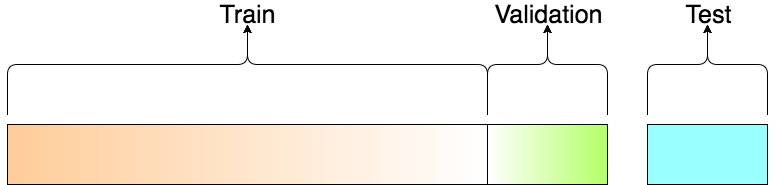
\includegraphics[width=.8\textwidth]{fig/train}
\end{frame}

\begin{frame}{Dataset categorization}
    \begin{enumerate}
        \item labeled vs.~unlabeled
            \begin{itemize}
                \item labeled
                    \begin{itemize}
                        \item the answer is known
                        \item e.g.~movie ratings
                        \item typically expensive to create
                        \item we could always use more of it
                        \item \emph{supervised learning}
                    \end{itemize}
                \item unlabeled
                    \begin{itemize}
                        \item the answer is unknown
                        \item cheaper, more plentiful
                        \item \emph{unsupervised learning}
                    \end{itemize}
            \end{itemize}
        \item continuous vs.~discrete
        \item categorical vs.~quantitative / numerical
    \end{enumerate}
\end{frame}

\begin{frame}{The data mining process}
    \begin{enumerate}
        \item Data collection
        \item Data cleaning
            \begin{itemize}
                \item noise and outlier filtering
                \item handling missing data
            \end{itemize}
        \item Data transformation / preprocessing
            \begin{itemize}
                \item dimensionality reduction (less used nowadays)
                \item normalization, standardization
            \end{itemize}
        \item Training the model
        \item Evaluating the model
    \end{enumerate}
\end{frame}

\begin{frame}{Learning types}
	\begin{itemize}
		\item \textbf{Supervised learning}
		\begin{itemize}
			\item is a problem where for every input variable(x) there is an ouput variable(y) in the training data
			\item the preparation of the output variables is usually done with Human resources - Labeled data
		\end{itemize}
		\item \textbf{Unsupervised learning}
		\begin{itemize}
			\item is a problem where only the input variable(x) is present in the training data
			\item still can be very useful since labeling data is very resource hungry and expensive
		\end{itemize}
	\end{itemize}
\end{frame}

\begin{frame}{Data mining problems 1.}
    \begin{itemize}
        \item Classification \visible<2->{-- \textcolor{darkred}{supervised, discrete classes}}
            \begin{itemize}
                \item assign a label for each sample
                \item labels are predefined and usually not very numerous
                \item e.g.~is an email a spam or a ham?
            \end{itemize}
        \item Regression \visible<3->{-- \textcolor{darkred}{supervised, continuous target}}
            \begin{itemize}
                \item predict a continuous variable
                \item e.g.~predict real estate prices, stock market based on history, location, amenities
            \end{itemize}
    \end{itemize}
\end{frame}

\begin{frame}{Data mining problems 2.}
    \begin{itemize}
        \item Clustering \visible<2->{-- \textcolor{darkred}{unsupervised, discrete clusters}}
            \begin{itemize}
                \item group samples into clusters according to a similarity measure
                \item goal: high intra-group similarity (samples in the same cluster should be similar to each other),
                    low inter-group similarity (samples in different clusters shouldn't be similar)
                \item e.g.~market segmentation
            \end{itemize}
    \end{itemize}
\end{frame}

\begin{frame}{Data mining problems 3.}
    \begin{itemize}
        \item Time series analysis and prediction
            \begin{itemize}
                \item pattern discovery and prediction in time series
            \end{itemize}
        \item Frequent itemset mining
            \begin{itemize}
                \item e.g.~What products do people buy at the same time?
            \end{itemize}
        \item Recommendation systems
            \begin{itemize}
                \item e.g.~movies similar to the ones the user already likes
            \end{itemize}
    \end{itemize}
\end{frame}


\begin{frame}{Classification vs. Clustering}
    \begin{center}
        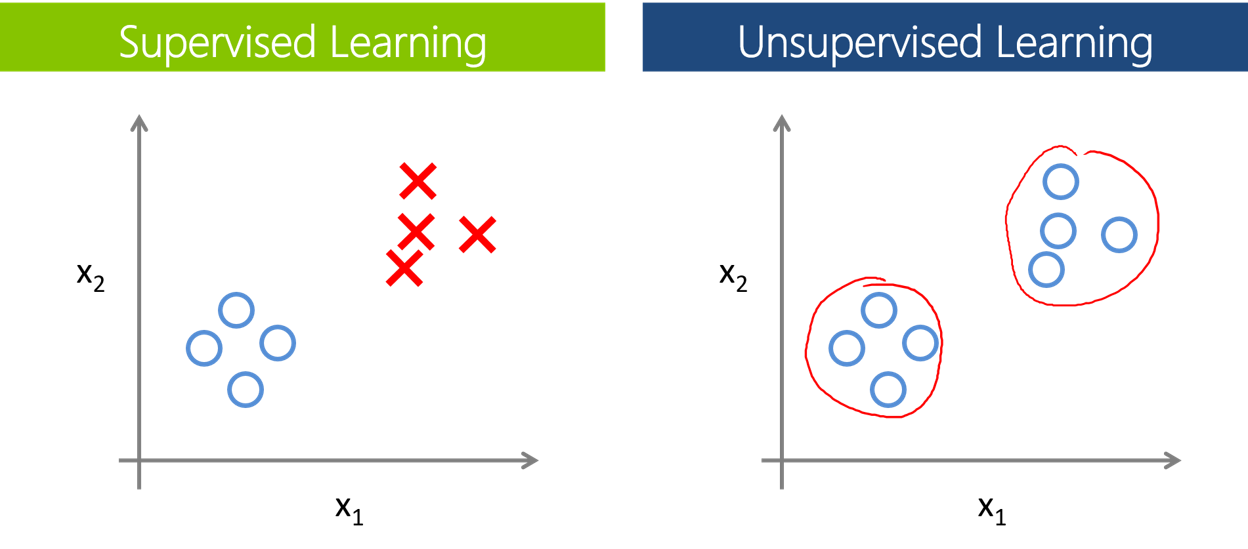
\includegraphics[width=.8\textwidth]{fig/sup_unsup.png}
    \end{center}
\end{frame}

\begin{frame}{Algorithms}
	\begin{itemize}
		\item Support vector machine (Classification, Regression)
		\item Decision Tree (Classification, Regression)
		\item Random Forest (Classification, Regression)
		\item Logistic Regression (Classification)
		\item Linear Regression (Regression)
		\item Neural Networks (Classification, Regression)
		\item K-means (Clustering)
		\item LDA (Clustering)
	\end{itemize}
\end{frame}

\begin{frame}{Evaluation - Binary classification}
    \begin{center}
\includegraphics[width=.8\textwidth]{true_pos}
    \end{center}
\end{frame}

\begin{frame}{Precision, recall and F-score}

{\bf Precision}: fraction of positive samples among those labeled positive
\begin{equation*}
	\text{Precision}=\frac{tp}{tp+fp}
\end{equation*}

{\bf Recall}: fraction of recovered positive samples of all positive samples
\begin{equation*}
	\text{Recall}=\frac{tp}{tp+fn}
\end{equation*}

\pause

{\bf F-score}: harmonic mean of precision and recall
    \begin{equation*}
        \text{F-score} = 2 * \frac{\text{prec}  \text{rec}}{\text{prec} + \text{rec}}
    \end{equation*}
\end{frame}

\begin{frame}{Evaluation - multiclass classification}
    \begin{itemize}
        \item one-versus-rest precision, recall and F-score
            \begin{itemize}
                \item samples from class $i$ are the positive, everything else are the negative examples
                \item $k$ scores for $k$ classes
            \end{itemize}
        \item average or weighted average of all $k$ scores
    \end{itemize}
\end{frame}

\begin{frame}{Evaluation - regression}
    Root-mean-square error

    \begin{equation*}
        \operatorname{RMSE}=\sqrt{\frac{\sum_{t=1}^n (\hat y_t - y_t)^2}{n}},
    \end{equation*}

    where $\hat y_t$ are the predicted values, $y_t$ is the true value and $n$ is the number of samples.
\end{frame}

\begin{frame}{Evaluation - clustering}
    \begin{itemize}
        \item high intra-cluster similarity, low inter-cluster similarity
        \item direct evaluation on the application of interest
        \item against gold standard labeled set
    \end{itemize}
\end{frame}

\begin{frame}{Technology}
    \begin{itemize}
        \item Python, R, Java, Lua
        \item Linux, Windows less so
        \item `traditional' machine learning: scikit-learn (Python), Weka (Java)
        \item deep learning: TensorFlow, PyTorch, Keras etc.
        \item plain text, CSV, TSV, XML (less popular)
    \end{itemize}
\end{frame}

\begin{frame}{AI - ML - DL differences}
    \begin{center}
        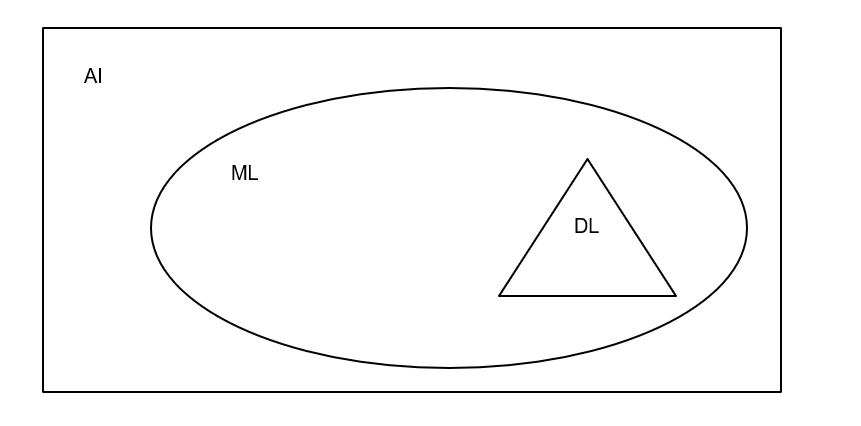
\includegraphics[width=.8\textwidth]{fig/ai_ml_dl.png}
    \end{center}
\end{frame}

\begin{frame}{ML vs DL}
    \begin{center}
        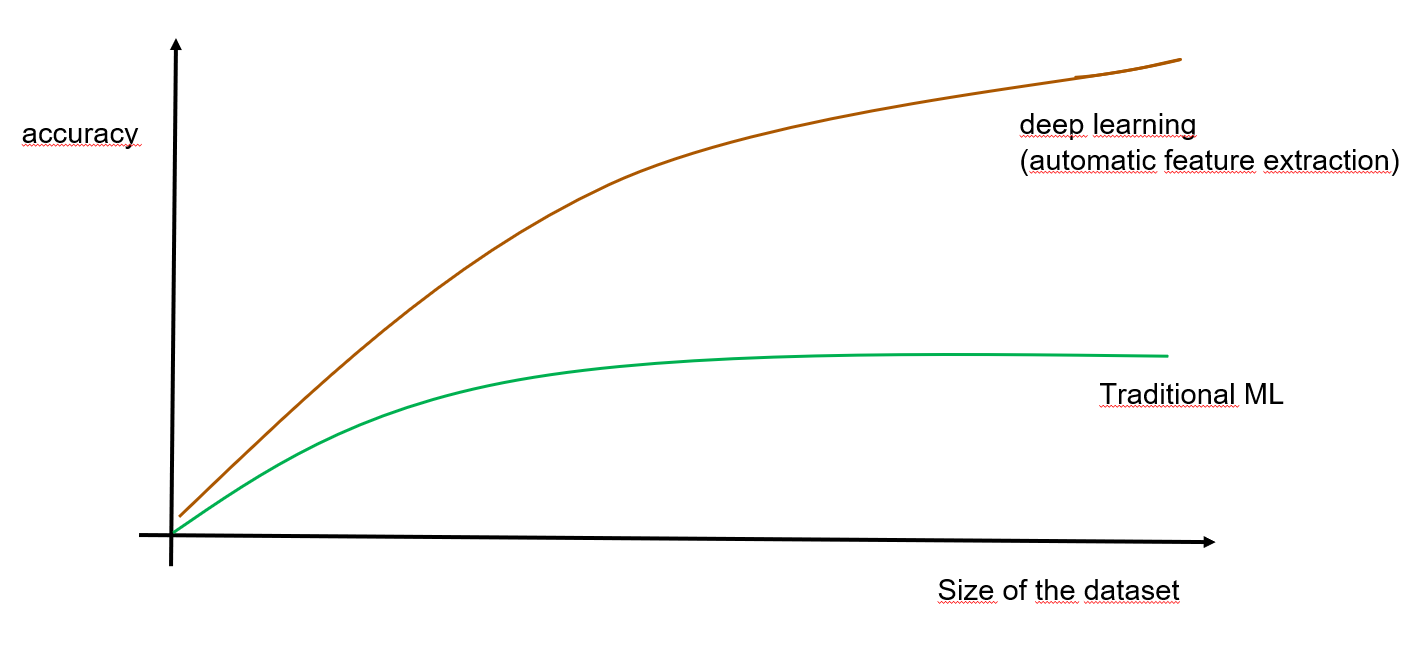
\includegraphics[width=.8\textwidth]{fig/ml_dl_scale.png}
    \end{center}
\end{frame}

\begin{frame}{Deep learning}
    \begin{itemize}
    	\item until now we talked about traditional Machine Learning
        \item representation learning instead of task-specific manual features
        \item biological inspiration (neurons, activation)
        \item why Deep learning returned?
        \begin{itemize}
        	\item fast GPU-s
        	\item good architectures
        	\item good methods
        \end{itemize}
    \end{itemize}
\end{frame}

\begin{frame}{Deep learning}
    \begin{itemize}
    	\item it has a black-box nature
        \item interpreting them is hard
        \item we don't exactly know the reasoning behind a decision
        \item can we trust Deep learning?
        \item the latest language model of \textbf{OpenAI}, GPT-3, has 175B trainable parameters \href{https://news.developer.nvidia.com/openai-presents-gpt-3-a-175-billion-parameters-language-model/}{link}
    \end{itemize}
\end{frame}

\begin{frame}{Terminology}
    \begin{itemize}
        \item How do ML/DL algorithms learn?
        \item \textbf{Loss function}:  helps to calculate the prediction loss of our network, which tells us how bad/good is our model.
        \item We want to \textbf{optimize} the loss/cost function.
        \item How?
            \begin{itemize}
                \item \textbf{Gradient descent} helps us find the global minima of the loss function
                \item \textbf{Backpropagation} algorithm is used to propagate the error back to the weights of the model and updates them
            \end{itemize}
    \end{itemize}   
\end{frame}

\begin{frame}{Under- and overfitting}
	
	\centering
    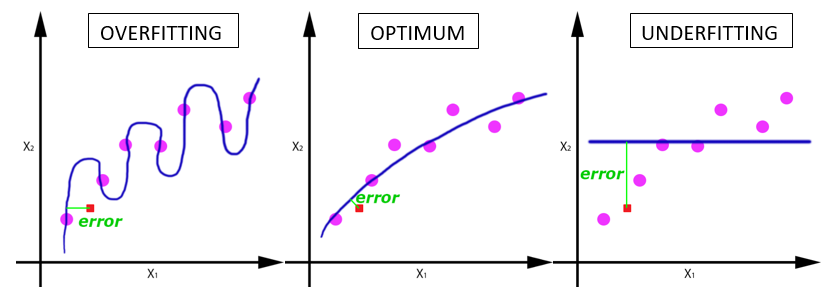
\includegraphics[width=.8\textwidth]{fig/underover.png}
    
    We use \textbf{Regularization} to avoid overfitting.
\end{frame}

\begin{frame}{ML vs Deep learning}
	
	\centering
	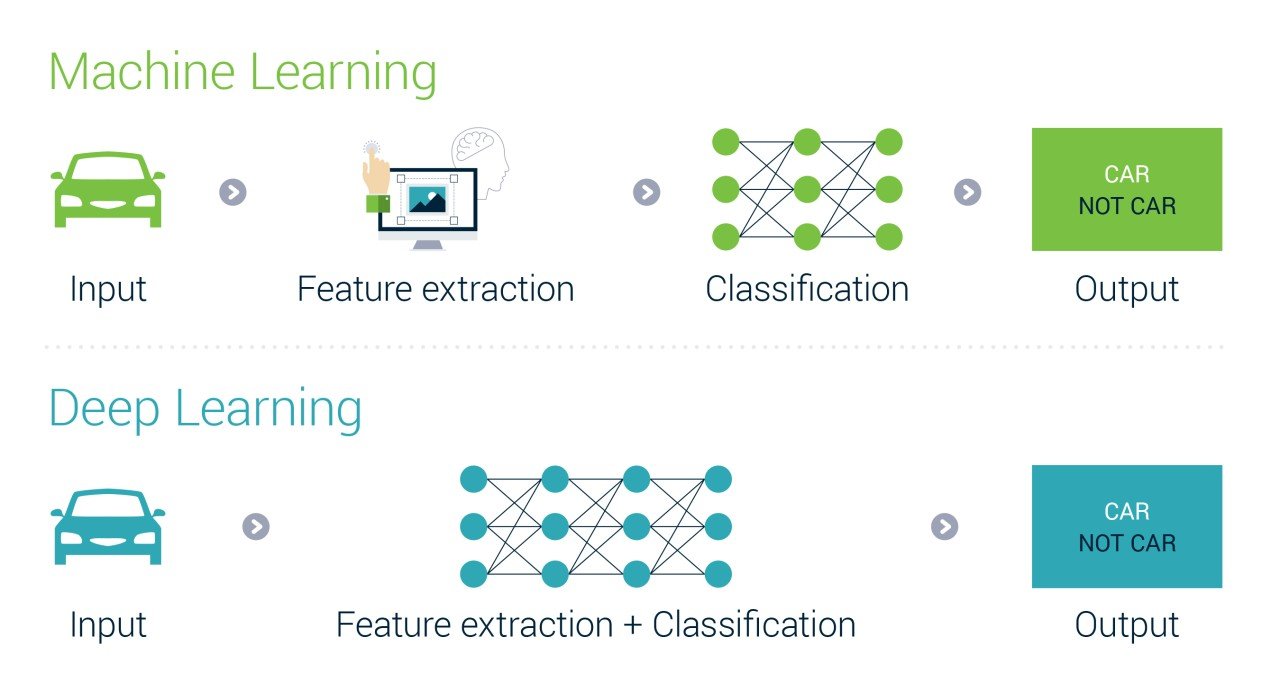
\includegraphics[width=.8\textwidth]{fig/ml}
\end{frame}


\begin{frame}{ML vs Deep Learning}
	\begin{itemize}
		\item \textbf{Deep learning}
		\begin{itemize}
			\item Automatic feature engineering
			\item Scalable with big data
			\item Can solve non-separable problems as well (traditional methods struggle with non-linearity)
			\item Currenlty most state-of-the-art methods are based on DL
		\end{itemize}
		\item \textbf{Traditional Machine Learning}
		\begin{itemize}
			\item Feature extraction is done manually
			\item Can learn realitvely well from small data (DL can't)
			\item Scalability is worse with big data
			\item It can be enough for small tasks
		\end{itemize}
	\end{itemize}
\end{frame}
\begin{frame}{Feed forward neural network}
    \def\layersep{2.1cm}

    \begin{tikzpicture}[shorten >=1pt,->,draw=black!50, node distance=\layersep]
        \tikzstyle{every pin edge}=[<-,shorten <=1pt]
        \tikzstyle{neuron}=[circle,fill=black!25,minimum size=17pt,inner sep=0pt]
        \tikzstyle{input neuron}=[neuron, fill=green!50];
        \tikzstyle{output neuron}=[neuron, fill=red!50];
        \tikzstyle{hidden neuron}=[neuron, fill=blue!50];
        \tikzstyle{annot} = [text width=3em, text centered]
    
        % Draw the input layer nodes
        \foreach \name / \y in {1,...,4}
        % This is the same as writing \foreach \name / \y in {1/1,2/2,3/3,4/4}
            \node[input neuron, pin=left:Input \#\y] (I-\name) at (0,-\y) {};
    
        % Draw the hidden layer nodes
        \foreach \name / \y in {1,...,5}
            \path[yshift=0.5cm]
                node[hidden neuron] (H-\name) at (\layersep,-\y cm) {};
    
        \foreach \name / \y in {15,25,35,45}
            \path[yshift=0.5cm]
                node[hidden neuron] (H-\name) at (\layersep+\layersep,-\y mm) {};
    
        % Draw the output layer node
                \node[output neuron,pin={[pin edge={->}]right:Output}] (O) at (3*\layersep, -25 mm) {};
    
        % Connect every node in the input layer with every node in the
        % hidden layer.
        \foreach \source in {1,...,4}
            \foreach \dest in {1,...,5}
                \path (I-\source) edge (H-\dest);
    
        % Connect every node in the hidden layer with the output layer
        \foreach \source in {1,...,5}
            \foreach \dest in {15,25,35,45}
                \path (H-\source) edge (H-\dest);
    
        \foreach \source in {15,25,35,45}
            \path (H-\source) edge (O);
    
        % Annotate the layers
        \node[annot,above of=H-1, node distance=1cm] (hl) {Hidden layer 1};
        \node[annot,right of=hl, node distance=\layersep] (hl2) {Hidden layer 2};
        \node[annot,left of=hl] {Input layer};
        \node[annot,right of=hl2] {Output layer};
    \end{tikzpicture}
\end{frame}

\begin{frame}{Feed forward neural network}
    \begin{equation*}
        \mathbf{h_1} = \sigma (\mathbf{W_1 x})
    \end{equation*}
    \begin{equation*}
        \mathbf{h_2} = \sigma (\mathbf{W_2 h_1})
    \end{equation*}
    \begin{equation*}
        \mathbf{y} = \sigma (\mathbf{W_3 h_2})
    \end{equation*}

$\sigma$: activation function, typically non-linear such as the sigmoid function
    \begin{equation*}
        \sigma(x) = \frac{1}{1 + e^{-x}}
    \end{equation*}

\end{frame}

\begin{frame}{Feed forward neural network}
    \begin{itemize}
        \item fixed input ($\mathbf{x}$) and output ($y$)
        \item weights are learned through backpropagation
        \item capacity or memory of the network
    \end{itemize}
    Drawbacks:
    \begin{itemize}
        \item data flows in one direction
        \item temporal and spacial relationships are not explicitly modeled
    \end{itemize}
\end{frame}

\begin{frame}{Recurrent neural network}
    \begin{itemize}
        \item the network has directed cycles
        \item temporal relationships are easier to learn
        \item Long-short term memory (LSTM)
            \begin{itemize}
                \item LSTM cells have \emph{memory}, can retain, update or forget previous information
                \item a network typically uses hundreds of these cells
            \end{itemize}
        \item Gated recurrent unit (GRU)
            \begin{itemize}
                \item memory cell similar to LSTM
            \end{itemize}
    \end{itemize}
\end{frame}

\begin{frame}{Convolutional neural network}
    \begin{itemize}
        \item spacial structures are explicitly modeled
        \item very successful in image processing
        \item can be applied to one dimensional data (1D convolution) such as text or audio
    \end{itemize}
\end{frame}

\begin{frame}{Other architectures}
    \begin{itemize}
        \item Generative adversarial network (GAN)
            \begin{itemize}
                \item two networks compete against each other: a generator and a discriminator
                \item generator: tries to create fake samples similar to real samples
                \item discriminator: tried to distinguish real samples from fake samples
                \item hard to train
                \item extremely popular, hundreds of variants
            \end{itemize}
    \end{itemize}
\end{frame}

\begin{frame}{Other architectures}
    \begin{itemize}
        \item (Variational) autoencoder (VAE)
            \begin{itemize}
                \item the input and the output of the network are the same
                \item the network learns to compress the input, then recover the original image from the compressed representation
                \item not very good at compression, but learns useful representation
                \item variational: generate real-like samples from noise
            \end{itemize}
    \end{itemize}
\end{frame}

\begin{frame}{Thank you for your attention}
	
\end{frame}
\end{document}
